% p10-06 例 3：正方形 ABCD 边长 4, E∈BC F∈CD, ∠EAF=45°, BE=1 → DF=12/5, CE=3, CF=8/5
% A(0,4), B(4,4), C(4,0), D(0,0)
\documentclass[tikz,border=4pt]{standalone}
\usepackage{ctex}
\usepackage{amsmath}
\usetikzlibrary{calc}
\begin{document}
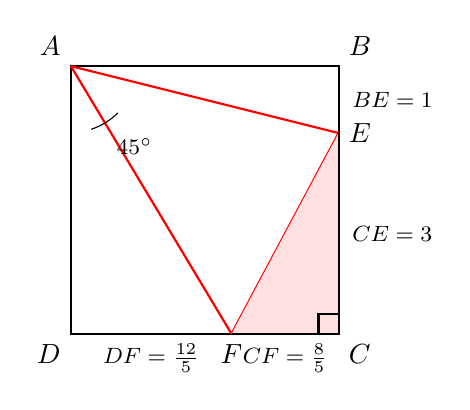
\begin{tikzpicture}[scale=0.85, thick]
  \coordinate (A) at (0,4);
  \coordinate (B) at (4,4);
  \coordinate (C) at (4,0);
  \coordinate (D) at (0,0);
  \coordinate (E) at (4,3);    % BE=1
  \coordinate (F) at (2.4,0);  % DF=12/5=2.4

  \draw (A)--(B)--(C)--(D)--cycle;
  \draw[red, thick] (A)--(E);
  \draw[red, thick] (A)--(F);
  \draw[red, thick] (E)--(F);

  % △CEF 阴影
  \fill[red!12] (C)--(E)--(F)--cycle;
  \draw (C)--(E);
  \draw (C)--(F);

  % 角 ∠EAF=45°
  \draw[thin] ($(A)+(0.7,-0.7)$) arc[start angle=-45, end angle=-72, radius=1.0];
  \node[font=\footnotesize] at (0.95, 2.8) {$45^\circ$};

  % ∠ECF 直角
  \draw ($(C)+(-0.3,0)$)--($(C)+(-0.3,0.3)$)--($(C)+(0,0.3)$);

  \node[above left]  at (A) {$A$};
  \node[above right] at (B) {$B$};
  \node[below right] at (C) {$C$};
  \node[below left]  at (D) {$D$};
  \node[right] at (E) {$E$};
  \node[below] at (F) {$F$};

  \node[font=\footnotesize, right] at (4.05, 3.5) {$BE=1$};
  \node[font=\footnotesize, right] at (4.05, 1.5) {$CE=3$};
  \node[font=\footnotesize, below] at (1.2, 0) {$DF=\tfrac{12}{5}$};
  \node[font=\footnotesize, below] at (3.2, 0) {$CF=\tfrac{8}{5}$};
\end{tikzpicture}
\end{document}
